\chapter{Nombres entiers naturels, récurrence et ensembles finis}
\minitoc
\minilof
\minilot
\label{chap:naturels}
\section{Nombres entiers naturels}

\subsection{Ensemble des naturels \(\N\)}

L'ensemble des entiers naturels \(\N=\{0,1,2,\ldots\}\) est muni de deux lois de compositions internes~: une addition notée \(+\) et d'une multiplication notée \(\times\) ou \(\cdot\) ou rien du tout qui vérifient les propriétés suivantes. On notera \(\N^*=\N\setminus\{0\}\).

\begin{prop}[Loi \(+\)]
  Elle est associative 
  \begin{equation}
    \forall (a,b,c) \in \N^3 \quad (a+b)+c=a+(b+c),
  \end{equation}
  commutative
  \begin{equation}
    \forall (a,b) \in \N^2 \quad a+b=b+a,
  \end{equation}
  l'entier \(0\) est son élément neutre
  \begin{equation}
    \forall a \in \N \quad a+0=0+a=a,
  \end{equation}
  et tout entier naturel est régulier pour cette loi
  \begin{equation}
    \forall (a,b,c) \in \N^3 \quad a+b=a+c \implies b=c.
  \end{equation}
\end{prop}
\begin{prop}[Loi \(\times\)]
  Elle est associative 
  \begin{equation}
    \forall (a,b,c) \in \N^3 \quad (a\times b)\times c=a\times (b\times c),
  \end{equation}
  commutative
  \begin{equation}
    \forall (a,b) \in \N^2 \quad a\times b=b\times a,
  \end{equation}
  distributive par rapport à la loi \(+\)
  \begin{equation}
    \forall (a,b,c) \in \N^3 \quad (a+ b)\times c=a\times c + b\times c,
  \end{equation}
  l'entier \(1\) est son élément neutre
  \begin{equation}
    \forall a \in \N \quad a\times 1=1\times a=a,
  \end{equation}
  et tout entier naturel non nul est régulier pour cette loi
  \begin{equation}
    \forall a \in \N^* \ \forall (b,c) \in \N^3 \quad a\times b=a\times c \implies b=c.
  \end{equation}
\end{prop}
On munit l'ensemble \(\N\) d'une relation d'ordre total notée \(\leqslant\) qui vérifie les propriétés suivantes
\begin{prop}
  Toute partie non vide de \(\N\) admet un plus petit élément et toute partie non vide et majorée de \(\N\) admet un plus grand élément.
\end{prop}
\begin{prop}
  La relation d'ordre \(\leqslant\) est compatible avec l'addition et la multiplication. C'est-à-dire que
  \begin{equation}
    \forall (a,b,c,d)\in \N^4 \quad
    \begin{cases}
      a\leqslant b \\ c \leqslant d
    \end{cases}
    \iff
    \begin{cases}
      a+c\leqslant b+d \\ ac\leqslant bd
    \end{cases}.
  \end{equation}
\end{prop}

 Si \(p\) et \(q\) sont des entiers naturels tels que \(p\leqslant q\) alors \(\intervalleentier{p}{q}= \N\cap\intervalleff{p}{q}\) 

\subsection{Théorème de récurrence}

\begin{theo}[théorème de récurrence]
  \label{theo:rec}
  Soient A une partie de \(\N\), et \(n_0\in\N\) tel que
  \begin{itemize}
  \item Initialisation~: \(n_0\in A\);
  \item Hérédité~: \(\forall n\geqslant n_0 \quad n\in A \implies n+1\in A\);
  \end{itemize}
  Conclusion~: Alors \(\forall n \in N \quad n\geqslant n_0 \implies n \in A\).
\end{theo}
\begin{proof}
  Soit \(E=\N\cap \intervallefo{n_0}{+\infty}\), l'ensemble des entiers plus grands ou égaux à \(n_0\) et \(B=\complement_E A\). Montrons par l'absurde que \(B\) est vide. 

Supposons que \(B\) soit non vide, alors il admet un plus petit élément noté \(\alpha\). Alors par définition de \(E\), \(\alpha\geqslant n_0\) ; et par hypothèse d'initialisation \(n_0\in A\), donc \(\alpha > n_0\), c'est-à-dire donc \(\alpha\geqslant n_0+1\geqslant 1\). Par suite \(\alpha-1\geqslant n_0\). 

Puisque \(\alpha\) est le plus petit élément de \(B\), \(\alpha-1 \notin B\) donc \(\alpha-1 \in A\). Alors par hypothèse d'hérédité, on obtient que \(\alpha-1+1=\alpha\in A\). 

L'hypothèse de départ qu'on avait fait nous disait que \(\alpha \in B\). L'élément \(\alpha\) ne peut être à la fois dans \(A\) et dans \(B\), on arrive donc à une absurdité, alors B est vide, \(E=A\).
\end{proof}
\begin{cor}[Récurrence simple]
  \label{cor:recsimple}
  Soit \(\P\) une propriété définie sur \(\N\cap \intervallefo{n_0}{+\infty}\) telle que
  \begin{itemize}
  \item Initialisation \(\P(n_0)\) est vraie;
  \item Hérédité \(\forall n\geqslant n_0 \quad \P(n) \implies \P(n+1)\);
  \end{itemize}
  Conclusion alors \(\forall n\geqslant n_0 \quad \P(n)\).
\end{cor}
\begin{proof}
  On applique le théorème de récurrence à \(A=\enstq{n\in\N}{\P(n)}\) puisque~:
  \begin{itemize}
  \item Initialisation \(\P(n_0) \iff n_0 \in A\)
  \item Hérédité
    \begin{equation}
      \left(\forall n\geqslant n_0 \quad \P(n) \implies \P(n+1)\right) \iff \left( \forall n \geqslant n_0 \quad n\in A \implies n+1\in A\right)
    \end{equation}
  \end{itemize}
  Conclusion alors d'après le théorème \(A=\N\cap \intervallefo{n_0}{+\infty}\)
\end{proof}
\begin{cor}[Récurrence double]
  \label{cor:recdouble}
  Soit P une propriété définie sur \(\N\cap \intervallefo{n_0}{+\infty}\) telle que
 \begin{itemize}
  \item Initialisation \(\P(n_0)\) et \(\P(n_1)\) sont vraie;
  \item Hérédité \(\forall n\geqslant n_0 \ \P(n)\) et \(\P(n+1) \implies \P(n+2)\);
  \end{itemize}
  Conclusion alors \(\forall n \in \N\cap \intervallefo{n_0}{+\infty} \ \P(n)\) 
\end{cor}
\begin{proof}
  On définit sur \(\N\cap \intervallefo{n_0}{+\infty}\) la propriété \(Q(n)=(\P(n) \text{ et } \P(n+1))\) et on applique le corollaire~\ref{cor:recsimple} à \(Q\).
\end{proof}
Il ne faut pas oublier d'initialiser deux fois. Il existe aussi des récurrences triples ou multiples, qu'il ne faut pas oublier d'initialiser autant de fois.
\begin{cor}[Récurrence forte]
  \label{cor:recforte}
  Soit P une propriété définie sur \(\N\cap \intervallefo{n_0}{+\infty}\) telle que
  \begin{itemize}
  \item Initialisation \(\P(n_0)\) est vraie;
  \item Hérédité \(\forall n \in \N\cap \intervallefo{n_0}{+\infty} \ (\P(n_0), \ldots, \P(n)) \implies \P(n+1)\)
  \end{itemize}
  Conclusion alors \(\forall n \in \N\cap \intervallefo{n_0}{+\infty}\ \ \P(n)\)
\end{cor}
\begin{proof}
  On définit sur \(\N\cap \intervallefo{n_0}{+\infty}\) la propriété \(R(n)=(\P(n_0), \ldots, \P(n))\) et on applique le corollaire~\ref{cor:recsimple} à \(R\).
\end{proof}

\subsection{Suites définies par une relation de récurrence}

Soit \(E\) un ensemble. On rappelle qu'une suite à valeur dans \(E\) est une famille d'éléments de \(E\) indexée par \(\N\). Étant donné \(a\in E\) et \(f\in E^E\), il existe une seule suite \((u_n)_{n\in\N}\) telle que (I) \(u_0=a\) et (H) \(u_{n+1}=f(u_n)\). C'est une conséquence du théorème de récurrence (théorème~\ref{theo:rec}).

De même on peut définir une unique suite \((u_n)_{n\in\N}\) par la donnée de~:
\begin{enumerate}
\item \(u_0, u_1\) deux éléments de \(E\) et une relation de récurrence de la forme \(u_{n+2}=f(u_{n+1},u_{n})\) avec \(f:E\times E\longmapsto E\) d'après le corollaire~\ref{cor:recdouble}.
\item \(u_0\) élément de \(E\) et une relation de récurrence de la forme \(u_{n+1}=f(n,u_{0},\ldots,u_{n})\) avec \(f:\N\times E^{n+1}\longmapsto E\) d'après le corollaire~\ref{cor:recforte}.
\end{enumerate}

\subsection{Exemples}
\begin{defdef}[Suite arithmétique]
  Une suite arithmétique à valeurs dans le corps des complexes \(\C\) est une suite définie par la donnée de \(u_0\in\C\) et d'une relation de récurrence 
  \begin{equation}
    \forall n \in \N \quad u_{n+1}=u_n+r
  \end{equation}
  où le complexe \(r\) est la raison et ne dépend pas de \(n\).
\end{defdef}
\begin{prop}
  Soit \(u\) une suite arithmétique de raison \(r\), alors
  \begin{equation}
    \forall n \in \N \quad u_n=u_0+nr.
  \end{equation}
\end{prop}
\begin{proof}
  Pour tout entier \(n\) on définit la propriété \(\P(n) \ u_n=u_0+nr\). On initialise et on voit que \(\P(0)\) est vraie. Ensuite on vérifie l'hérédité : soit un entier \(n\) et on suppose que \(\P(n)\) est vraie, alors \(u_{n+1}=u_n+r\) par définition et \(u_{n+1}=u_0+(n+1)r\) par hypothèse de récurrence, donc \(\P(n+1)\) est vraie. Alors d'après le théorème de récurrence la proposition est vraie.
\end{proof}
\begin{prop}
  Soit \(u\) une suite arithmétique de premier terme \(a\in\C\) et de raison \(r\in\C\), alors pour tout entier \(n\)
  \begin{equation}
    S_n=\sum_{k=0}^n u_k=(n+1)a+r\frac{n(n+1)}{2}.
  \end{equation}
\end{prop}
\begin{proof}
  Soit un entier \(n\), alors
  \begin{equation}
    S_n=\sum_{k=0}^n u_0+kr= \sum_{k=0}^n u_0 + r\sum_{k=0}^n k.
  \end{equation}
  On montre par récurrence que \(\sum_{k=0}^n k=\frac{n(n+1)}{2}\), en effet pour \(n=0\) \(\sum_{k=0}^0 k=0=\frac{0(0+1)}{2}\) et pour l'hérédité si on considère que la somme est vraie pour un entier \(n \geqslant 1\) alors \(\sum_{k=0}^{n+1} k= n+1 \sum_{k=0}^n k=n+1+\frac{n(n+1)}{2}=\frac{(n+2)(n+1)}{2}\).
\end{proof}
\begin{defdef}[Suite géométrique]
  Une suite géométrique à valeur dans \(\C\) est une suite définie par la donnée de \(u_0\in\C\) et d'une relation de récurrence
  \begin{equation}
    \forall n \in \N \quad u_{n+1}=ru_n,
  \end{equation}
  où \(r\in\C\) est la raison de la suite et ne dépend pas de \(n\).
\end{defdef}
\begin{prop}
  Soit \(u\) une suite géométrique de raison \(r\), alors
  \begin{equation}
    \forall n \in \N \quad u_n=u_0r^n.
  \end{equation}
\end{prop}
\begin{proof}
  Soit pour tout \(n\in\N\) la propriété \(\P(n)\ u_n=u_0r^n\). On remarque que \(\P(0)\) est vraie puisque \(r^0=1\). Soit un naturel \(n\geqslant 1\) et supposons que \(\P(n)\) soit vraie. Alors \(u_{n+1}=r u_n\) par définition et par hypothèse de récurrence \(u_{n+1}=r u_n = r u_0 r^n=u_0 r^{n+1}\) donc \(\P(n+1)\) est vraie. Par théorème de récurrence pour tout entier \(n\in\N\) \(\P(n)\) est vraie.
\end{proof}
\begin{prop}
  Soit \(u\) une suite géométrique de premier terme \(u_0\in\C\) et de raison \(r\in\C\). Soient \(p\) et \(q\) deux entiers naturels tels que \(p\leqslant q\), alors
  \begin{equation}
    S_{p,q}=\sum_{k=p}^q u_k=
    \begin{cases}
      (q-p+1) & r=1 \\
      \frac{u_p-u_{q+1}}{1-r}=u_0r^p\left(\frac{1-r^{q-p+1}}{1-r}\right) & r \neq 1
    \end{cases}.
  \end{equation}
  C'est ``le premier terme écrit'' moins ``le premier terme négligé'' sur ``un moins la raison''.
\end{prop}
\begin{proof}
  Si \(r=1\) alors \(S_{p,q}=\sum_{k=p}^qu_0=(q-p+1)u_0\) et sinon on a
  \begin{align}
    (1-r)S_{p,q}=(1-r)\sum_{k=p}^q u_0r^k &= \sum_{k=p}^q u_0r^k - \sum_{k=p}^q u_0r^{k+1}\\
&=\sum_{k=p}^q u_0r^k - \sum_{j=p+1}^{q+1} u_0r^{j}\\
&=u_0 r^p -u_0 r^{q+1} = u_p-u_{q+1},
  \end{align}
et puisque \(r\neq 1\) on a bien  \(S_{p,q}=\frac{u_p-u_{q+1}}{1-r}\).
\end{proof}
\begin{prop}
  Soient \(a\) et \(b\) deux complexes et \(n\) un entier naturel, alors
  \begin{equation}
    a^{n+1}-b^{n+1}=(a-b)\sum_{k=0}^n a^k b^{n-k}.
  \end{equation}
\end{prop}
\begin{proof}
  \begin{itemize}
  \item si \(a=b\) la proposition est vraie puisque \(0=0\);
  \item si \(a=0\) alors \(-b^{n+1}=-b b^n\);
  \item si \(a\neq 0\) et \(a\neq b\), on définit la suite géométrique \(u\) de premier terme \(1\) et de raison \(\frac{b}{a}\) qui existe puisque \(a\neq 0\) et qui est différente de \(1\) puisque \(a\neq b\). En appliquant la proposition précédente on a~: 
\begin{equation}
  S_{0,n}=\sum_{k=0}^n\left(\frac{b}{a}\right)^k=\frac{1-\left(\frac{b}{a}\right)^{n+1}}{1-\frac{b}{a}},
\end{equation}
donc
\begin{equation}
  a^n \sum_{k=0}^n\left(\frac{b}{a}\right)^k = \frac{a^{n+1}-b^{n+1}}{a-b},
\end{equation}
finalement
\begin{equation}
  (a-b)\sum_{k=0}^n b^ka^{n-k}=(a-b)\sum_{k=0}^n b^{n-k}a^{k}=a^{n+1}-b^{n+1}.
\end{equation}
\end{itemize}
On peut aussi le démontrer directement en utilisant les sommes télescopiques comme dans le calcul de \(S_{p,q}\).
\end{proof}

\section{Entiers naturels \(n!\) et \(\binom{n}{k}\)}

\subsection{Factorielle}

\begin{defdef}
  Pour tout entier naturel \(n\) non nul, on définit \(n!=\prod_{k=1}^n k\) et par convention \(0!=1\).
\end{defdef}
\begin{prop}
  La suite \((n!)_{n\in\N}\) est l'unique suite \(u\) vérifiant
  \begin{equation}
    \begin{cases}
      u_0=1 \\
      \forall n\geqslant 1 \quad u_{n+1}=(n+1) u_n
    \end{cases}.
  \end{equation}
\end{prop}
\begin{proof}
  L'unicité est assurée par le théorème de récurrence. 
\end{proof}
Quelques valeurs de la factorielle sont données par le tableau \ref{tab:factorielle}. Cette suite croît très vite, plus vite que l'exponentielle.
\begin{table}[h]
    \centering
    \begin{tabular}{|c|c|c|c|c|c|c|c|c|c|}
        \hline
        0 & 1 & 2 & 3 & 4  & 5   & 6   & 7    & 8     & 9 \\ \hline
        1 & 1 & 2 & 6 & 24 & 120 & 720 & 5040 & 40320 & 362880 \\ \hline
    \end{tabular}
    \caption{Premières valeurs de la factorielle}
    \label{tab:factorielle}
\end{table}

\subsection{Coefficients binomiaux -- formule de Pascal}

\begin{defdef}[Coefficients binomiaux]
  Pour tout entier naturels \(n\) et \(p\) on définit un nombre noté \(\binom{n}{p}\) par~:
  \begin{equation}
    \begin{cases}
      \binom{n}{p}=\frac{n!}{p!(n-p)!} & 0\leqslant p \leqslant n \\
      \binom{n}{p}=0 & p > n
    \end{cases}.
  \end{equation}
\end{defdef}
\begin{prop}
  Soit un entier naturel \(n\), alors \(\binom{n}{0}=1\), \(\binom{n}{1}=n\) et \(\binom{n}{2}=\frac{n(n-1)}{2}\).
\end{prop}
\begin{proof}
  \begin{gather}
    \forall n \in \N \quad \binom{n}{0}=\frac{n!}{0!(n-0)!}=1; \\
    \forall n \in \N \ \forall m\in \N^* \quad \binom{m}{1}=\frac{m!}{1!(m-1)!}=m \ \binom{0}{1}=0;\\
    \forall n \geqslant 2 \quad \binom{n}{2}=\frac{n!}{2!(n-2)!}=\frac{n(n-1)}{2} \ \binom{0}{2}=\binom{1}{2}=0.
  \end{gather}
\end{proof}
\begin{prop}
  \begin{gather}
    \forall (n,p)\in\N^2 \quad 0\leqslant p \leqslant n \quad \binom{n}{p}=\binom{n}{n-p};\\
    \forall (n,p)\in\N\times\N^* \quad \binom{n}{p}=\frac{n}{p}\binom{n-1}{p-1} \quad \binom{n}{p}=\frac{n-p+1}{p}\binom{n}{p-1};
  \end{gather}
  \begin{equation}
      \label{eq:TrianglePascal}
    \forall (n,p)\in{\N^*}^2 \ \binom{n}{p}=\binom{n-1}{p-1}+\binom{n-1}{p}.
  \end{equation}
  Une représentation graphique est donnée en figure \ref{fig:TrianglePascal}\footnote{Crédit : https://www.logamaths.fr/} pour illustrer cette dernière formule.
\end{prop}
\begin{proof}
  \begin{enumerate}
  \item Il faut et il suffit de changer \(n\) par \(n-p\) dans la définition;
  \item soient \((p,n)\in\N^2\ p\neq 0\) alors~:
    \begin{itemize} 
    \item si \(p>n\) alors \(\binom{n}{p}=0\) et \(p-1>n-1\) alors \(\binom{n-1}{p-1}=0\) d'où l'égalité, si \(0<p\leqslant n\) alors
      \begin{align}
        \binom{n}{p}=\frac{n!}{p!(n-p)!}&=\frac{n}{p}\frac{(n-1)!}{(p-1)!((n-1)-(p-1))!}\\
        &=\frac{n}{p}\binom{n-1}{p-1}
      \end{align}
    \item si \(p>n\) \(\binom{n}{p}=0\) alors \(p-1\geqslant n\) et si \(p-1=n\) alors \(n-p+1=0\) et les deux membres de l'égalité sont nuls; si \(p-1>n\)  \(\binom{n}{p-1}=0\) et les deux membres de l'égalité sont nuls.
    \item si \(0<p<n\) alors
      \begin{align}
        \binom{n}{p}&=\frac{n-p+1}{p}\frac{n!}{(p-1)!(n-p+1)(n-p)!}\\
        &=\frac{n-p+1}{p}\frac{n!}{(p-1)!(n-p+1)!}
      \end{align}
      donc \(\binom{n}{p}=\frac{n-p+1}{p}\binom{n}{p-1}\)
    \end{itemize}
  \item Soient \(n\) et \(p\) deux entiers tout deux non nuls, alors
    \begin{itemize}
    \item si \(p>n\) alors \(p>p-1>n-1\) alors \(\binom{n}{p}=0=0+0=\binom{n-1}{p-1}+\binom{n-1}{p}\)
    \item si \(0<p\leqslant n-1\) alors \(p<n\) et \(p-1<n-1\) donc
      \begin{align}
        \binom{n-1}{p}+\binom{n-1}{p-1}&=\frac{(n-1)!}{p!(n-1-p)}+\frac{(n-1)!}{(p-1)!((n-1)-(p-1))!}\\
        &=\frac{(n-1)!}{(p-1)!(n-1-p)!}\left(\frac{1}{p}+\frac{1}{n-p}\right)\\
        &=\frac{(n-1)!}{(p-1)!(n-1-p)!}\frac{n}{p(n-p)}\\
        &=\frac{n!}{p!(n-p)!}=\binom{n}{p}
      \end{align}
    \item si \(p=n\) alors
      \begin{equation}
        \binom{n-1}{p}+\binom{n-1}{p-1}=\binom{n-1}{n}+\binom{n-1}{n-1}=0+1=\binom{n}{n}.
      \end{equation}
    \end{itemize}
  \end{enumerate}
\end{proof}
\begin{figure}
    \centering
    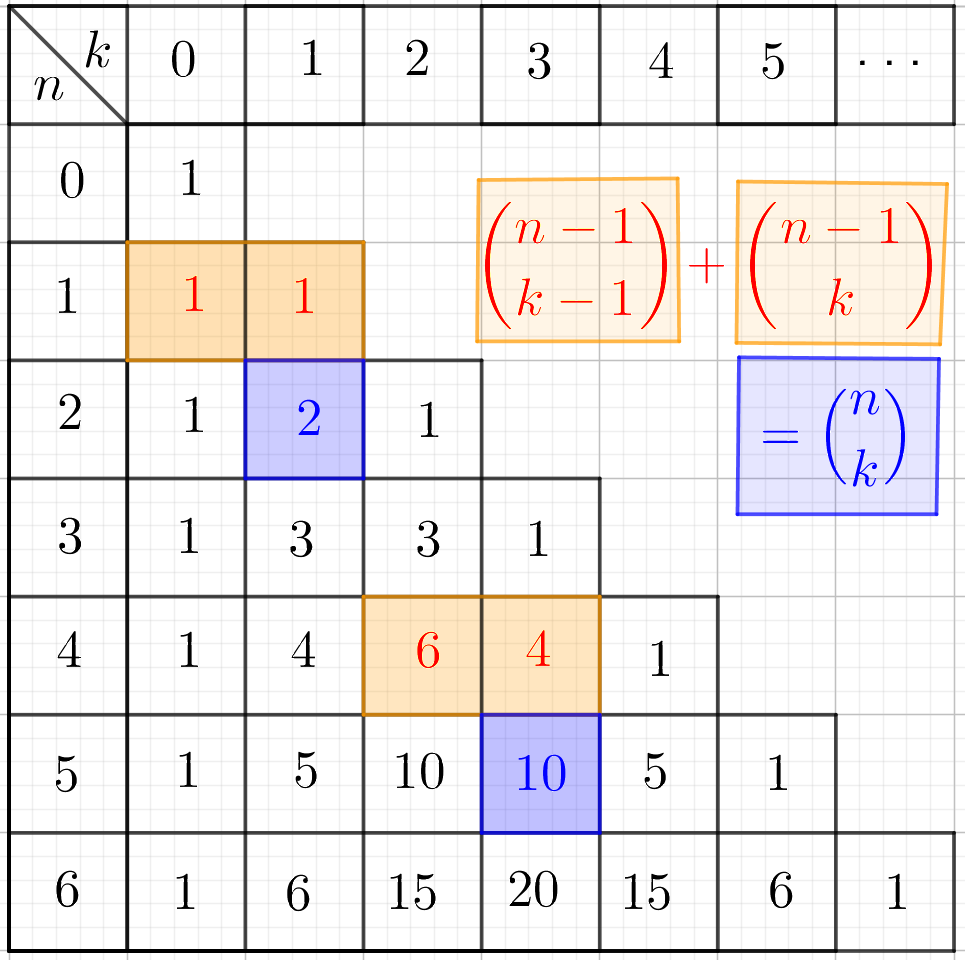
\includegraphics[scale=0.7]{./Triangle-de-Pascal-01-3.png}
    \caption{Représentation --- Triangle de Pascal --- de la formule \eqref{eq:TrianglePascal}}
    \label{fig:TrianglePascal}
\end{figure}
\begin{prop}
  Soient deux entiers naturels \(n\) et \(p\), alors \(\binom{n}{p}\) est un entier naturel.
\end{prop}
\begin{proof}
  On démontre ce résultat par récurrence sur \(n\in\N\). On définit la propriété \(\P(n)\) ``\(\forall p \in \N \ \binom{n}{p}\in\N\)''. On vérifie l'étape d'initialisation \(n=0\) : \(\binom{0}{p}=\begin{cases} 0 & p>0 \\ 1 & p=1\end{cases}\) donc \(\P(0)\) est vraie. 
  
Vérifions l'hérédité, soit \(n \in \N\) et supposons que \(\P(n)\) soient vraie, alors \(\binom{n+1}{0}=1\in \N\). Pour tout \(p\) non nul \(\binom{n+1}{p}=\binom{n}{p}+\binom{n}{p-1}\) d'après la relation de Pascal. L'hypothèse de récurrence donne \(\binom{n}{p}\in\N\) et \(\binom{n}{p-1}\in\N\) et puisque l'addition est une loi de composition interne sur \(\N\) alors \(\binom{n+1}{p}\in\N\). Donc \(\P(n+1)\) est vraie. 

Le théorème de récurrence nous permet de conclure et de dire que la proposition \(\P(n)\) est vraie pour n'importe quel entier naturel \(n\).
\end{proof}

\subsection{Formules du binôme de Newton}

\begin{prop}
  Pour tous complexes \(a\) et \(b\) et tout entier \(n\),
  \begin{equation}
    (a+b)^n=\sum_{k=0}^n \binom{n}{k}a^kb^{n-k}.
  \end{equation}
  On peut aussi voir que les coefficients de la décomposition du binôme de Newton peuvent être visualisés sur les lignes du triangle de Pascal, voir la figure \ref{fig:TrianglePascal}.
\end{prop}
\begin{proof}
  Soient \(a\),\(b\) deux complexes et \(n\) un entier naturel, alors on définit la propriété \(\P(n)\) ``\((a+b)^n=\sum_{k=0}^n \binom{n}{k}a^kb^{n-k}\)''. Vérifions l'étape initiale~:
\begin{equation}
  (a+b)^0=1=\binom{0}{0}a^0b^0=\sum_{k=0}^0 \binom{0}{k}a^kb^{0-k},
\end{equation}
\(\P(0)\) est vraie. Vérifions ensuite l'hérédité en supposant que \(\P(n)\) soit vraie alors
\begin{align}
  (a+b)^n&=(a+b)(a+b)^n=(a+b)\sum_{k=0}^n \binom{n}{k}a^kb^{n-k}\\
  &=\sum_{k=0}^n \binom{n}{k}a^{k+1}b^{n-k}+\sum_{k=0}^n \binom{n}{k}a^kb^{n-k+1}\\
  &=\sum_{j=1}^{n+1} \binom{n}{j-1}a^{j}b^{n-j+1}+\sum_{k=0}^n \binom{n}{k}a^kb^{n-k+1}\\
  &=\binom{n}{n}a^{n+1}b^0 +\binom{n}{0}a^0b^{n+1} + \sum_{k=1}^{n}\left[\binom{n}{k-1}+\binom{n}{k}\right]a^kb^{n+1-k}\\
  &=\binom{n+1}{n+1}a^{n+1}b^0+\binom{n+1}{0}a^0b^{n+1}+ \sum_{k=1}^{n}\binom{n+1}{k}a^kb^{n+1-k}\\
  &=\sum_{k=0}^{n+1}\binom{n+1}{k}a^kb^{n+1-k}.
\end{align}
Donc \(\P(n+1)\) est vraie.

Le théorème de récurrence nous permet donc de conclure et d'affirmer que pour tout entier \(n\) la proposition \(\P(n)\) est vraie.
\end{proof}
Cas particulier :
\begin{equation}
  \sum_{k=0}^n \binom{n}{k}=2^n.
\end{equation}

\section{Ensembles finis -- dénombrement}

\subsection{Notion d'ensemble fini}

\begin{defdef}
  Soit \(E\) un ensemble. \(E\) est fini s'il existe un entier \(n\) non nul et une bijection \(\varphi:\intervalleentier{1}{n} \longmapsto E\), sinon \(E\) est infini.
\end{defdef}
\begin{theo}\label{theo:ensemblefini}
  Soient \(p\) et \(q\) deux entiers naturels non nuls. S'il existe une bijection \(\varphi:\intervalleentier{1}{p} \longmapsto \intervalleentier{1}{q}\) alors \(p=q\).
\end{theo}
\begin{proof}
  Hors programme, cependant la démonstration est écrite en annexe~\ref{chap:ensemblesFinis}.
\end{proof}
\begin{prop}[Définition]
  Soit \(E\) un ensemble fini. Alors l'entier naturel \(n\) de la définition est unique et on l'appelle le cardinale de \(E\) et on le note \(\Card E\).
\end{prop}
Par convention, l'ensemble vide est fini et son cardinal vaut \(0\).
\begin{proof}
  Soient deux bijections \(\varphi:\intervalleentier{1}{n} \longmapsto E\) et \(\psi:\intervalleentier{1}{p} \longmapsto E\) (on note \(\psi^-1:E \longmapsto \intervalleentier{1}{p}\)). Par composé de deux bijections, l'application \(\psi^-1\circ \varphi: \intervalleentier{1}{n} \longmapsto \intervalleentier{1}{p}\) est une bijection. Si on applique le théorème~\ref{theo:ensemblefini} on en déduit donc que \(n=p\).
\end{proof}
\begin{prop}
  Soit \(E\) un ensemble fini et \(F\) un ensemble tel qu'il existe une bijection \(\varphi:E\longmapsto F\). alors \(F\) est un ensemble fini de même cardinal que \(E\).
\end{prop}
\begin{proof}
  \(E\) est fini, donc il existe un entier \(n\) et une bijection \(\psi:\intervalleentier{1}{n} \longmapsto E\). Ainsi l'application \(\varphi\circ\psi:\intervalleentier{1}{n} \longmapsto F\) est bijective, puisque c'est la composée de deux applications bijectives. Donc \(F\) est un ensemble fini et \(\Card F=n=\Card E\).
\end{proof}

Si \(E\) est un ensemble fini de cardinal \(n\neq 0\), l'existence d'une bijection \(\varphi:\intervalleentier{1}{n} \longmapsto E\) permet de ``numéroter'' les éléments de \(E\) et donc d'écrire l'ensemble \(E\) en extension \(E=\{\varphi(1), \ldots, \varphi(n)\}\).
Réciproquement, si on dispose d'une écriture en extension on peut en déduire que \(E\) est un ensemble fini mais pas forcément que son cardinal est égal à \(p\), car pour cela il faut que les éléments soient distincts.

La notion de cardinal correspond à la notion intuitive du nombre d'éléments d'un ensemble.

\subsection{Parties finies}

\subsubsection{Parties finies de \(\N\)}

\begin{theo}\label{theo:partfinN}
  Soit \(\P\) une partie non vide et majorée de \(\N\). Alors il existe un entier non nul \(n\) et une bijection croissante \(\varphi:\intervalleentier{1}{n} \longmapsto \P\). \(\P\) est donc fini et de plus le couple \((n,\varphi)\) est unique.
\end{theo}
\begin{proof}
  La démonstration est hors programme, elle se fait par récurrence sur \(M\in\N^*\) et la propriété est \(\P(M)\) Pour toute partie non vide \(\P\) de \(\N\) et majorée par M, il existe un unique couple \((n,\varphi)\) avec \(n\neq 0\) et \(\varphi:\intervalleentier{1}{n} \longmapsto \P\) bijective et croissante. 
\end{proof}

\begin{enumerate}
\item La définition de la fonction \(\varphi\) correspond à l'idée de ranger les éléments par ordre croissant;
\item L'application \(\varphi:\intervalleentier{1}{n} \longmapsto \P\) \(\P \subset \N\) est telle que \(\varphi(1)\geqslant 0\) \(\varphi(2)\geqslant 1\) \ldots;
\item On montre par récurrence que pour tout \(k\in\intervalleentier{1}{n} \ \varphi(k)\geqslant k-1\), en particulier \(\varphi(n)\leqslant n-1\). 

Or \(M\) est un majorant de \(\P\) donc \(\varphi(n)\leqslant M\) donc \(n-1\leqslant M\) soit alors \(n\geqslant M+1\).
\item M est un majorant de \(\P\) donc \(\varphi(n)\geqslant M\) et \(\varphi\) est strictement croissante donc \(\varphi(n-1)<\varphi(n)\) donc \(\varphi(n-1)\leqslant\varphi(n)-1\) donc \(\varphi(n-1)\leqslant M-1\). 

On montre par récurrence descendante sur \(k\in\intervalleentier{0}{n}\) la propriété \(\P(k) \ \varphi(k)\leqslant M-(n-k)\)

Initialisation à n : \(\P(n)\) est vraie puisque \(\varphi(n)\leqslant M\).

Hérédité : Supposons \(\P(k)\) vraie pour tout entier \(k\in\{2, \ldots,n\}\) et montrons alors que \(\P(k-1)\) est vraie. Puisque \(\varphi\) est strictement croissante, on a \(\varphi(k-1)\leqslant \varphi(k)-1\) et par hypothèse de récurrence \(\P(k)\) est vraie donc \(\varphi(k)\leqslant M-(n-k)\) et \(\varphi(k-1)\leqslant M-(n-k)-1=M-(n-k+1)=M-(n-(k-1))\) donc \(\P(k-1)\) est vraie. 

On en conclue donc , grâce au théorème de récurrence, que la proposition est vraie. \(\forall k \in \{1, \ldots, n\} \varphi(k)\leqslant M-(n-k)\). Si \(n=M+1\) alors 
\(k-1\leqslant \varphi(k)\leqslant M - (M+1-k)=k-1\) donc \(\forall k \in \{1, \ldots,n\} \varphi(k)=k-1\) et ainsi \(\P=\varphi(\intervalleentier{1}{n})=\intervalleentier{0}{n-1}= \intervalleentier{0}{M}\).
\end{enumerate}
\begin{prop}
  Soit \(\P\) une partie non vide de \(\N\). Alors \(\P\) est finie si et seulement si\(\P\) est majorée.
\end{prop}
\begin{proof}
  \begin{itemize}
  \item[\(\impliedby\)] Déjà fait grâce au théorème~\ref{theo:partfinN}.
  \item[\(\implies\)] On démontre par récurrence sur \(p=\Card(\P)\in \N^*\) la propriété \(\P(p)\) pour toute partie finie \(\P\) de \(\N\), si \(\P\) est de cardinal \(p\) alors \(\P\) est majorée. 

Regardons l'initialisation à \(p=1\), si \(\P\) est de cardinal \(1\), il existe un entier \(a\in\N\) tel que \(\P=\{a\}\) et \(a\) est un majorant de \(\P\) donc \(\P\) est majorée.

Ensuite, passons à l'hérédité. Soit \(p \in \N\) et supposons que \(\P(p)\) soit vérifiée. Soit une partie \(\P\) de \(\N\) à \(p+1\) éléments, alors soit \(a\in \P\) et \(\P'=\P\setminus\{a\}\). La partie \(\P'\) est une partie de \(\N\) à \(p\) éléments, donc d'après l'hypothèse de récurrence elle et majorée. Notons \(M\) le majorant de \(\P'\) et notons \(N=\max(M,a)\). Alors \(N\) est un majorant de la partie \(\P\). La partie \(\P\) est donc majorée. \(\P(p+1)\) est donc vérifiée.

Grâce au théorème de récurrence, on peut affirmer que la propriété \(\P(p)\) est vraie sur \(N^*\). Donc une partie finie de \(\N\) est majorée.
  \end{itemize}
\end{proof}

\subsubsection{Parties d'un ensemble fini}

\begin{theo}\label{theo:partiesfinies}
  Soient \(E\) et F deux ensembles tel que \(E\) soit fini et \(F\subset E\). Alors F est un ensemble fini et \(\Card(F)\leqslant\Card(E)\). De plus \(F=E \iff \Card(F)=\Card(E)\)
\end{theo}
\begin{proof}
  \begin{enumerate}
  \item Si \(F=\emptyset\), \(F\) est fini et son cardinal est nul, \(0\leqslant\Card(E)\). De plus \(E=F=\emptyset \iff \Card(E)=0=\Card(F)\);
  \item sinon il existe un entier \(n\) non nul tel qu'il existe une bijection \(\varphi:\intervalleentier{1}{n} \longmapsto E\). Soit \(A=\varphi^{-1}(F) \subset\intervalleentier{1}{n}\). A est une partie non vide et majorée de \(\N\). A est donc une partie finie de \(\N\). Il existe donc un entier naturel \(p\) non nul et une bijection \(\psi:\intervalleentier{1}{p} \longmapsto A\). On peut définir la restriction \(\fonction{\widetilde{\varphi}}{A}{F}{x}{\varphi(x)}\). \(\widetilde{\varphi}\) est bijective. En effet~:
    \begin{itemize}
    \item \(\widetilde{\varphi}\) est injective, puisque si pour tout \(x,y\) de A \(\widetilde{\varphi}(x)=\widetilde{\varphi}(y)\) alors \(\varphi(x)=\varphi(y)\) et comme \(\varphi\) est injective (puisque bijective) on a \(x=y\).
    \item \(\widetilde{\varphi}\) est surjective, pour tout \(y\in F\) il existe \(x\in E\) tel \(y\varphi(x)\). Mais \(A=\varphi^{-1}(F)\) donc \(x\in A\) et \(y=\varphi(x)=\widetilde{\varphi}(x)\).
    \end{itemize}
    Soit \(f=\widetilde{\varphi}\circ \psi\), alors \(f\) est bijective comme la composée de deux applications bijectives. On a prouvé que F est un ensemble fini de cardinal p. Soit \(A'=\{x-1, x\in A\}\subset \N\). \(A'\) est une partie finie de \(\N\) de même cardinal que \(A\) et donc que \(F\). Puisque \(A\subset\intervalleentier{1}{n}\) alors \(A'\subset\intervalleentier{0}{n-1}\). \(M=n-1\) est un majorant de \(A'\). Alors \(p=\Card(A')\leqslant M+1=n-1+1=n\). De plus, 
    \begin{itemize}
    \item si \(E=F\) alors \(\Card(E)=\Card(F)\)
    \item si \(\Card(E)=\Card(F)\), alors \(n=p=M+1\) on en déduit que \(A'=\intervalleentier{0}{M} = \intervalleentier{0}{n-1}\) et donc que \(A=\intervalleentier{1}{M+1} = \intervalleentier{1}{n}\). \(F=\varphi(A)=\varphi(\intervalleentier{1}{n})=E\)
    \end{itemize}
  \end{enumerate}
\end{proof}

Si \(E\) est un ensemble infini, \(E\) peut par exemple être en bijection avec une de ces parties strictes. Comme par exemple \(\N\) et l'ensemble des entiers pairs sont en bijection.

\subsection{Opérations sur les ensembles finis}

\subsubsection{Réunion d'ensembles finis}

\begin{prop}\label{prop:reunionfindis}
  Soient \(E\) et F deux ensembles finis \emph{disjoints}. Alors \(E\cup F\) est fini et 
  \begin{equation}
    \Card(E\cup F)=\Card(E)+\Card(F).
  \end{equation}
\end{prop}

\begin{proof}
  Soit \(n=\Card(E)\geqslant 1\) et \(m=\Card(F)\geqslant 1\). Il existe deux bijections \(\varphi\) et \(\psi\) telles que \(\varphi:\intervalleentier{1}{n} \longmapsto E\) et \(\psi:\intervalleentier{1}{m} \longmapsto F\). Soit maintenant l'application
  \begin{equation}
    \fonction{f}{\intervalleentier{1}{m+n}}{E\cup F}{k}{\begin{cases} \varphi(k) & 1\leqslant k\leqslant n \\ \psi(k-n) & n+1\leqslant k\leqslant m+n\end{cases}}.
  \end{equation}
  Alors~:
    \begin{itemize}
    \item la fonction \(f\) est bien définie puisque si \(1\leqslant k \leqslant n\) alors \(\varphi(k)\) existe et \(\varphi(k)\in E\subset E\cup F\). si \(n+1\leqslant k \leqslant n+m\) alors \(1\leqslant k-n \leqslant m\) et donc \(\psi(k-n)\) existe et \(\psi(k)\in F\subset E\cup F\).
    \item la fonction \(f\) est injective. En effet, soient deux entiers \(k\) et \(k'\) différents  dans \(\intervalleentier{1}{m+n}\). Alors trois cas se proposent à nous~:
      \begin{itemize}
      \item si ces deux entiers sont dans \(\intervalleentier{1}{n}\), alors puisque \(\varphi\) est injective alors \(f\) l'est aussi.
      \item si ces deux entiers sont dans \(\intervalleentier{n}{n+m}\), alors puisque \(\psi\) est injective alors \(f\) l'est aussi.
      \item par contre si par exemple \(k\in\intervalleentier{1}{n}\) et \(k'\in\intervalleentier{n+1}{n+m}\) (on peut inverser les positions) alors \(f(k)=\varphi(k')\in E\) et \(f(k')=\psi(k'-n)\in F\) et \(E\cap F = \emptyset\) donc \(f(k)\neq f(k')\) donc \(f\) est aussi injective.
      \end{itemize}
    \item La fonction \(f\) est surjective. En effet, soit un élément \(y\) de \(E\cup F\). Si \(y\in E\), alors il existe un entier \(k\) dans \(\intervalleentier{1}{n}\) tel que \(y=\varphi(k)=f(k)\) puisque \(\varphi\) est surjective. Si \(y\in F\), alors il existe un entier \(k\) dans \(\intervalleentier{1}{n}\) tel que \(y=\psi(k)=f(k+n)\) puisque \(\psi\) est surjective. Donc \(f\) est surjective.
    \end{itemize}
    Au final, on a démontré que l'application \(f\) est bijective, donc \(E\cup F\) est un ensemble fini avec \(\Card(E\cup F)=n+m=\Card(E)+\Card(F)\).
  \end{proof}
  \begin{prop}
    Soient \(E\) et \(F\) deux ensembles finis, alors \(E\cup F\) est un ensemble fini et
    \begin{equation}
    \Card(E\cup F)=\Card(E)+\Card(F)-\Card(E\cap F).
  \end{equation}
\end{prop}
\begin{proof}
  On sait que 
  \begin{equation}
    E=(E\cap F)\cup (E\cap \bar{F}) \quad \emptyset=(E\cap F)\cap (E\cap \bar{F}),
  \end{equation} 
  alors en appliquant la proposition précédente on a
  \begin{equation}
    \Card(E)=\Card(E\cap F)+\Card(E\cap \bar{F}).
  \end{equation}
  Montrons que \(E\cup F =(E\cap \bar{F}) \cup F\). D'une part \(E \cap \bar{F} \subset E\) donc \((E\cap \bar{F}) \cup F \subset E\cup F\). D'autre part, soit un élément \(x\), alors si \(x \in \)E\( \cup F\) trois cas de figure se présentent~:
  \begin{itemize}
  \item si \(x\in F\) alors \(x \in (E\cap \bar{F}) \cup F\);
  \item si \(x \in E\) et \(x \in F\) alors \(x \in (E\cap \bar{F}) \cup F\);
  \item si \(x \in E\) et \(x \notin F\) alors \(x \in E\cap \bar{F}\), donc \(x \in (E\cap \bar{F}) \cup F\).
  \end{itemize}
  Alors \(E\cup F \subset (E \cap \bar{F})\cup F\), donc avec les deux inclusions \(E\cup F =(E\cap \bar{F}) \cup F\). On a aussi \((E\cap \bar{F})\cap F=\emptyset\), donc en appliquant la proposition~\ref{prop:reunionfindis}, \(E\cup F\) est un ensemble fini et
  \begin{align}
    \Card(E\cup F)&=\Card(E\cap \bar{F})+\Card(F)\\ &=\Card(E) - \Card(E\cap F)+\Card(F).
  \end{align}
\end{proof}
\begin{prop}
  Si \(F\) est une partie d'un ensemble fini \(E\), alors \(F\) est fini, son complémentaire \(\complement_E F\) est aussi fini et \(\Card(\complement_E F)=\Card(E)-\Card(F)\).
\end{prop}
\begin{proof}
  En appliquant le théorème~\ref{theo:partiesfinies}, les ensembles \(F\) et \(\complement_E F\) sont finis et comme ils sont disjoints de réunion égale à \(E\), la proposition~\ref{prop:reunionfindis}, nous permet d'écrire que
  \begin{equation}
    \Card(E)=\Card(F)+\Card(\complement_E F).
  \end{equation}
\end{proof}
\begin{prop}
  Soient \(p\) un entier naturel et \((A_k)_{k\in\intervalleentier{1}{p}}\) \(p\) ensembles deux à deux disjoints. Alors \(\bigcup_{k=1}^{p}A_k\) est un ensemble fini et
  \begin{equation}
    \Card\left(\bigcup_{k=1}^{p}A_k\right)=\sum_{k=1}^{p}\Card(A_k).
  \end{equation}
\end{prop}
\begin{proof}
  On démontre par récurrence sur \(p\in \N^*\) la propriété \(\P(p)\) ``pour toute suite d'ensemble \((A_k)_{k\in\intervalleentier{1}{p}}\) \(p\) ensembles deux à deux disjoints. Alors \(\bigcup_{k=1}^{p}A_k\) est un ensemble fini et \(\Card\left(\bigcup_{k=1}^{p}A_k\right)=\sum_{k=1}^{p}\Card(A_k)\)''. L'étape initiale pour \(p=1\) est évident. L'hérédité se démontre en supposant que pour un naturel \(p\), \(\P(p)\) vraie. On note \(B_p=\bigcup_{k=1}^{p}A_k\) et donc \(\bigcup_{k=1}^{p+1}A_k=A_{p+1}\cup B_p\). Puisque \(\P(p)\) est vraie, alors \(B_p\) est fini de cardinal \(\Card(B_p)=\sum_{k=1}^{p}\Card(A_k)\). Puisque tous les ensembles \((A_k)_{k\in\intervalleentier{1}{p+1}}\) sont deux à deux disjoints on a \(A_{p+1}\cap B_p=\emptyset\). D'après la proposition~\ref{prop:reunionfindis}, \(A_{p+1}\cup B_p\) est fini et
\begin{equation}
  \Card(A_{p+1}\cup B_p) = \Card(A_{p+1})+\Card(B_p).
\end{equation}
Donc si on remplace \(B_p\) par l'union on obtient
\begin{equation}
  \Card\left(\bigcup_{k=1}^{p+1}A_k\right) = \sum_{k=1}^{p+1}\Card(A_k).
\end{equation}
Donc \(\P(p+1)\) est vraie. Alors le théorème de récurrence nous permet de conclure en affirmant que la propriété P est vraie pour tout naturel \(p\) non nul.
\end{proof}

\subsubsection{Produit d'ensembles finis}
\begin{prop}\label{prop:produitfini}
  Soient \(E\) et \(F\) deux ensembles finis, alors \(E\times F\) est un ensemble fini et
  \begin{equation}
    \Card(E\times F)=\Card(E)\times \Card(F).
  \end{equation}
\end{prop}
\begin{proof}
Si \(E=\emptyset\) alors \(E\times F=\emptyset\) est finie et \(\Card(E\times F)=0=\Card(E)\times \Card(F)\).
  
Si \(E\neq\emptyset\), alors il existe un entier naturel non nul \(n\) et une application bijective \(\varphi:\intervalleentier{1}{n}\longmapsto E\). Donc on peut noter \(E=\{\varphi(1),\ldots ,\varphi(n)\}\) et \(A_k=\{\varphi(k)\}\times F\). Alors \(E\times F=\bigcup_{k=1}^n A_k\). Puisque \(\varphi\) est bijective, les \(A_k\) sont deux à deux disjoints. Soit pour tout \(k\in\intervalleentier{1}{n}\), \(\fonction{\psi_k}{F}{A_k}{x}{(\varphi(k),x)}\). Cette fonction est bien définie, elle est bijective. Donc \(A_k\) est un ensemble fini et \(\Card(A_k)=\Card(F)\). Puisque les \(A_k\) sont finis et deux à deux disjoints, le produit \(E\times F\) est fini et d'après la proposition~\ref{prop:reunionfindis} on a
    \begin{equation}
      \Card(E\times F)=\sum_{k=1}^{n} A_k=\sum_{k=1}^{n}\Card(F)=n\Card(F)=\Card(E)\times \Card(F).
    \end{equation}
\end{proof}
\begin{prop}
  Soit \(E\) un ensemble fini, alors pour tout entier naturel \(p\) non nul \(E^p\) est un ensemble fini et
  \begin{equation}
    \Card(E^p)=\Card(E)^p.
  \end{equation}
\end{prop}
\begin{proof}
  La démonstration se fait par récurrence sur \(p\in\N^*\), \(\P(p)\) ``\(E^p\) est fini et \(\Card(E^p)=\Card(E)^p\)''. L'étape d'initialisation, pour \(p=1\) est triviale. L'hérédité se démontre en considérant que pour tout naturel \(p\geqslant 1\), \(\P(p)\) vraie pour montrer \(\P(p+1)\). En effet puisque \(E^{p+1}=E^p \times E\) d'après l'hypothèse de récurrence \(E^p\) est fini et \(\Card(E^p)=\Card(E)^p\). La proposition~\ref{prop:produitfini} affirme que \(E^{p+1}\) est fini et que
  \begin{equation}
    \Card(E^{p+1})=\Card(E^p)\times \Card(E)=\Card(E)^{p+1}.
  \end{equation}
  Donc \(\P(p+1)\) est vraie. Ainsi par théorème de récurrence la proposition \(\P(p)\) est vraie pour tout entier \(p\) non nul.
\end{proof}

\subsection{Applications d'un ensemble fini vers un ensemble fini}
Soient \(E\) et \(F\) deux ensembles finis. On s'intéresse à l'ensemble des applications de \(E\) dans \(F\) noté \(F^E\).
\begin{theo}\label{theo:bijinjsurj}
  Soient \(E\) et F deux ensembles finis non vides \emph{de même cardinal} et \(f\in F^E\), alors
  \begin{equation}
    f \text{~est bijective}\iff f \text{~est injective}\iff f \text{~est surjective}.
  \end{equation}
\end{theo}
\begin{proof}
  On sait déjà que la bijectivité entraîne l'injectivité et la surjectivité.
  \begin{itemize}
  \item Supposons que \(f\) est injective. Soit \(A=f(E)\), l'application \(f^{|A}\) est une application bijective, donc \(\Card(A)=\Card(E)\) et puisque \(E\) et F ont le même cardinal, \(\Card(A)=\Card(F)\) mais on sait aussi que \(A\subset F\) donc au final \(A=f(E)=F\). Cela signifie que \(f\) est surjective. Elle est donc bijective (\(f^{|A}=f\)).
  \item Supposons que \(f\) est surjective. Pour tout \(y\in F\) on peut choisir un élément \(x\in E\) tel que \(y=f(x)\). Définissons l'ensemble \(A\) constitué par ces éléments \(x\) de E. L'application \(f_{|A}:A\longmapsto E\) est donc bijective. Alors \(\Card(A)=\Card(F)\) et puisque \(E\) et F ont le même cardinal, \(\Card(A)=\Card(E)\), or \(A\subset E\) donc \(A=E\) et ainsi \(f\) est bijective (\(f_{|A}=f\)).
  \end{itemize}
\end{proof}
\begin{itemize}
\item Si \(E\) et F sont finis de même cardinal, il existe une bijection \(\varphi:E\longmapsto F\). En effet il existe un entier naturel non nul \(n\) et une fonction \(f_1:\intervalleentier{1}{n} \longmapsto E\) bijective (puisque \(E\) est fini) et une fonction \(f_2:\intervalleentier{1}{n} \longmapsto F\) bijective (puisque \(F\) est fini), donc il faut et il suffit de prendre \(\varphi=f_2\circ f_1^{-1}\).
\item Si \(E\) et \(F\) sont finis et une application \(f:E\longmapsto F\), alors
  \begin{gather}
    f \text{~est injective} \implies \Card(E)\leqslant\Card(F); \\
    f \text{~est surjective}\implies \Card(E)\geqslant\Card(F);\\
    f \text{~est bijective} \implies \Card(E)=\Card(F). 
  \end{gather}
\end{itemize}
\begin{theo}
  Soient \(E\) et \(F\) des ensembles finis non vides, alors \(F^E\) est un ensemble fini tel que
  \begin{equation}
    \Card\left(F^E\right)=\Card(F)^{\Card(E)}.
  \end{equation}
\end{theo}
\begin{proof}
  Puisque \(E\) est fini, il existe un entier naturel \(p\) non nul et une bijection \(\varphi:\intervalleentier{1}{p} \longmapsto E\), c'est à dire qu'on peut écrire \(E=\{\varphi(k)\}_{k\in\intervalleentier{1}{p}}\). Soit l'application \(f\) telle que
  \begin{equation}
    \fonction{f}{F^E}{F^p}{u}{(u(\varphi(1)), \ldots, u(\varphi(p)))}.
  \end{equation}
  Alors \(f\) est bien définie : puisque pour toute fonction \(u\) de \(F^E\) et tout entier \(i\) de \(\intervalleentier{1}{p}\), \(\varphi(i) \in E\) et \(u(\varphi(i))\in F\). La fonction \(f\) est bijective, puisque pour tout \((b_1, \ldots, b_p) \in F^P\) il existe une unique application \(u:E\longmapsto F\) telle que \(u(\varphi(1))=b_1\), \ldots, \(u(\varphi(p))=b_p\). Alors \(F^E\) est fini et \(\Card\left(F^E\right)=\Card(F^p)=\Card(F)^p=\Card(F)^{\Card(E)}\).
\end{proof}
\begin{prop}\label{prop:nbinj}
  Soient \(E\) et F des ensembles finis non vide de cardinaux respectifs \(p\) et \(n\). Soit \(I(E,F)\) l'ensemble des injections de \(E\) dans F. Alors \(I(E,F)\) est fini et
  \begin{equation}
    \Card(I(E,F))=\prod_{k=0}^{p-1}(n-k)=n(n-1) \dotsm (n-p+1).
  \end{equation}
\end{prop}
\begin{proof}
  Notons \(A_n^p\) le nombre d'injections d'un ensemble à \(p\) éléments sur un ensemble à \(n\) éléments. On fait une récurrence sur le cardinal de l'ensemble de départ. Soit \(p\) un entier naturel non nul, alors \(\P(p)\) ``\(\forall n \in \N^* \ A_n^p=\prod_{k=0}^{p-1}(n-k)\)''. 
  \begin{itemize}
  \item[I] Si \(\Card(E)=1\) alors \(E=\{a\}\) donc \(I(E,F)=F^E\) puisque toutes les applications de \(E\) dans F sont injectives. Donc pour tout naturel non nul \(n\) \(A_n^1=\Card(F)^{\Card(E)}=n^1=n=\prod_{k=0}^{1-1}(n-k)\). Donc \(\P(1)\) est vérifiée.
  \item[H] Supposons que \(\P(p)\) soit vraie pour tout \(p\) non nul, alors soit \(E\) un ensemble fini de cardinal \(p+1\). Soit un entier naturel non nul \(n\) et F un ensemble de cardinal \(n\). Soit un élément \(a\in E\) et \(E'=E\setminus\{a\}\). Se donner une injection \(i\) de \(E\) dans F revient à se donner
    \begin{itemize}
    \item \(i(a)\) un élément de \(F\) (\(n=\Card(F)\) choix possibles),
    \item une application injective de \(E'\) sur \(F\setminus\{i(a)\}\) (\(A_{n-1}^p\) choix possibles d'après l'hypothèse de récurrence).
    \end{itemize}
    Donc \(A_{n}^{p+1}=n \times A_{n-1}^p\). Alors 
    \begin{itemize}
    \item si \(n\geqslant 2\), alors  \(A_{n-1}^p=\prod_{k=0}^{p-1}(n-1-k)\) et on a
      \begin{equation}
        A_{n}^{p+1}=n\prod_{k=0}^{p-1}(n-1-k)=\prod_{k=0}^{p}(n-k);
      \end{equation}
    \item si \(n=1\), alors \(A_{1}^{p+1}=0\) et \(\prod_{k=0}^{p}(1-k)=0\) car \(p\geqslant 1\).
    \end{itemize}
    On a montré que pour tout entier naturel \(n\) non nul, \(A_{n}^{p+1}=\prod_{k=0}^{p}(n-k)\). Donc \(\P(p+1)\) est vraie.
  \item[C] Par théorème de récurrence, \(\P(p)\) est vraie pour tout entier naturel \(p\) non nul.
  \end{itemize}
\end{proof}
\begin{defdef}
  Une permutation d'un ensemble \(E\) est une bijection de \(E\) dans E. On note \(\sigma(E)\) leur ensemble.
\end{defdef}
\begin{prop}
  Si \(E\) est un ensemble fini, \(\sigma(E)\) est un ensemble fini et
  \begin{equation}
    \Card(\sigma(E))=\prod_{k=0}^{n-1}(n-k)=n!.
  \end{equation}
\end{prop}
\begin{proof}
  En appliquant le théorème~\ref{theo:bijinjsurj} puisque \(E\) est fini et en notant que \(\sigma(E)=I(E,E)\) puis en appliquant la proposition~\ref{prop:nbinj} et on obtient
  \begin{equation}
    \Card(\sigma(E))=\prod_{k=0}^{n-1}(n-k)=n!.
  \end{equation}
\end{proof}

\subsection{Parties à \(p\) éléments d'un ensemble fini}

Soit \(E\) un ensemble fini. On note pour tout entier naturel \(p\), \(\Part_p(E)\) l'ensemble des parties de \(E\) à \(p\) éléments.
\begin{prop}\label{prop:ppartiesfinies}
  Soit \(E\) un ensemble fini de cardinal \(n\in \N\) et \(p \in \N\) alors \(\Part_p(E)\) est un ensemble fini et
  \begin{equation}
    \Card(\Part_p(E))=\binom{n}{p}
  \end{equation}
\end{prop}
\begin{proof}
  \begin{itemize}
  \item si \(p=0\) alors \(\Part_p(E)=\{\emptyset\}\) et \(\Card(\Part_p(E))=1=\binom{n}{0}\);
  \item si \(p>n\) alors \(\Part_p(E)=\emptyset\) et \(\Card(\Part_p(E))=0=\binom{n}{0}\);
  \item si \(1\leqslant p \leqslant n\) alors le nombre d'injection de \(\intervalleentier{1}{p}\) dans \(E\) est \(A_{n}^p=\frac{n!}{(n-p)!}\). Se donner une injection de  \(\intervalleentier{1}{p}\) dans \(E\) revient à
    \begin{itemize}
    \item choisir \(p\) éléments distincts dans E, c'est à dire une partie à \(p\) éléments de \(E\) (\(\Card(\Part_p(E))\) choix possibles);
    \item ordonner ces éléments, c'est à dire définir une bijection de \(\intervalleentier{1}{p}\) dans \(E\) (\(p!\) choix possibles).
    \end{itemize}
    Ainsi,
    \begin{equation}
      \frac{n!}{(n-p)!}=\Card(\Part_p(E)) p!.
    \end{equation}
    Du coup
    \begin{equation}
      \Card(\Part_p(E))=\binom{n}{p}.
    \end{equation}
  \end{itemize}
\end{proof}
\begin{defdef}
  Soit \(E\) un ensemble fini. On appelle combinaison de \(E\) à \(p\) éléments tout élément A de \(\Part_p(E)\).
\end{defdef}
\begin{prop}
  Soit \(E\) un ensemble fini, alors l'ensemble des parties de \(E\) \(\Part(E)\) est un ensemble fini et
  \begin{equation}
    \Card(\Part(E))=2^{\Card(E)}.
  \end{equation}
\end{prop}
\begin{proof}
  Soit \(n=\Card(E)\in \N\). Alors \(\Part(E)=\bigcup_{k=0}^{n}\Part_k(E)\), les \(\Part_k(E)\) sont tous deux à deux disjoints, donc d'après le théorème~\ref{theo:partiesfinies} et la proposition~\ref{prop:ppartiesfinies} on a
  \begin{equation}
    \Card(\Part(E))=\sum_{k=0}^n \Card(\Part_k(E))=\sum_{k=0}^n \binom{n}{k}=2^n.
  \end{equation}
\end{proof}
\section{Exercices}
\subsection{Raisonnement par récurrence}
\begin{exercice}
    Montrer, par récurrence (sans le binôme de Newton) que pour tout réel \(x \geqslant 0\) et tout entier naturel \(n\), \((1+x)^n \geqslant 1 + nx\).
\end{exercice}
\begin{exercice}
    Soit un naturel \(n\) non nul. Démontrer par récurrence les égalités suivantes (qui seront à connaître)~:
    \begin{flalign*}
        \sum_{k=1}^{n} k   & = \frac{n(n+1)}{2} \\
        \sum_{k=1}^{n} k^2 & = \frac{n(n+1)(2n+1)}{6}\\
        \sum_{k=1}^{n} k^3 & = \left(\frac{n(n+1)}{2}\right)^2
    \end{flalign*}
\end{exercice}
\begin{exercice}
    Montrer par récurrence les inégalités suivantes~:
    \begin{flalign*}
        \forall n \in \N^{*} \quad 2^{n-1} \leqslant n! \leqslant n^n \\
        \forall n \in \N^{*} \quad (n+1)! \geqslant \sum_{k=1}^{n} k!
    \end{flalign*}
\end{exercice}
\begin{exercice}
    Démontrer que pour tout naturel \(n\) et tout réel \(x\) \[\sin^{(n)}(x) = \sin\left(x + n\frac{\pi}{2}\right) \qquad \cos^{(n)}(x) = \cos\left(x + n\frac{\pi}{2}\right)\]
\end{exercice}
\begin{exercice}
    Soient les nombres \(C(n,p)\) définis par~:\[\begin{cases} C(0,0)=1 \\ \forall n \in \N^* C(n,0)=1 \\ \forall p \in \N^* C(0,p) = 0 \\ \forall (n,p) \in (\N^*)^2 C(n,p) = C(n-1,p) = C(n-1,p-1) \end{cases}\]
    Démontrer que pour tout naturels \(n\) et \(p\), \(C(n,p) = \binom{n}{p}\).
\end{exercice}
\begin{exercice}
    Trouver les applications \(f : \N \longmapsto \N\) strictement croissantes telles que~:
    \[\begin{cases} f(2) &= 2 \\\forall p, q \in \N, \ f(pq) &= f(p)f(q) \end{cases}\]
\end{exercice}
\begin{exercice}
    Soit une application \(f : I \longmapsto \R\) solution de l'équation différentielle \(y' = \cos^2(y)\). Démontrer que \(f\) est indéfiniment dérivable sur \(I\) et que pour tout \(x \in I\) et tout naturel \(n\) non nul~: \[f^{(n)}(x) = (n-1)! \cos^n(f(x)) \sin\left(nf(x) + n\frac{\pi}{2}\right)\]
\end{exercice}
\subsection{Sommation, ensembles finis}
\begin{exercice}
    Soit un naturel non nul \(n\). On pose \(p = E(n/2)\) et \(q = E((n-1)/2)\), où \(E\) désigne la partie entière. Déterminer une expression simple de chacune des sommes suivantes.
    \begin{align*}
        A_n &= \sum_{k=0}^n \binom{n}{k}, & B_n&=\sum_{k=0}^n (-1)^k\binom{n}{k}, & C_n&=\sum_{k=0}^p \binom{n}{2k}, \\
        D_n &= \sum_{k=0}^q \binom{n}{2k+1}, & E_n&=\sum_{k=0}^p (-1)^k\binom{n}{2k}, & F_n&=\sum_{k=0}^q (-1)^k\binom{n}{2k+1}, \\
        G_n &= \sum_{k=0}^n k\binom{n}{k}, & H_n&=\sum_{k=0}^n k(k-1)\binom{n}{k}, & I_n&=\sum_{k=0}^n k^2\binom{n}{k}
    \end{align*}
\end{exercice}
\begin{exercice}
    \begin{enumerate}
        \item Soient \(p, q, n\) des entiers naturels. Déterminer une expression simple de la somme \[\sum_{k=0}^n \binom{p}{k}\binom{q}{n-k}.\] Indication~: \((1+x)^{p+q} = (1+x)^p (1+x)^q\).
        \item En déduire une expression simple de \[\sum_{k=0}^n \binom{n}{k}^2\]
    \end{enumerate}
\end{exercice}
\begin{exercice}
    Pour tous naturels \(n\) et \(p\) tels que \(n \leqslant p\), on pose \(S(n,p) = \sum_{k=n}^p \binom{k}{n}\).
    \begin{enumerate}
        \item Démontrer que \(S(n,p) = \binom{p+1}{n+1}\)
        \item Soit \(p \geqslant 1\). En utilisant cette expression, retrouver les expressions bien connues de~:\[\sum_{k=1}^p k ; \sum_{k=1}^p k^2 ; \sum_{k=1}{p} k^3\]
    \end{enumerate}
\end{exercice}
\begin{exercice}
    Soient \(A, B, C\) trois parties d'un ensemble \(E\). Exprimer le cardinal de \(A \cup B \cup C\) en fonction des cardinaux de \(A, B, C\) et de leurs intersections.
\end{exercice}
\begin{exercice}
    Soient deux naturels non nuls \(n\geqslant p\). Quel est le nombre d'applications strictement croissantes de \(\intervalleentier{1}{p}\) dans \(\intervalleentier{1}{n}\) ?
\end{exercice}
\begin{exercice}
    Soient \(E\) un ensemble fini de cardinal \(n\) et \(A\) une partie de \(E\) de cardinal \(p\).
    \begin{enumerate}
        \item Quel est le nombre de parties à \(k\) éléments de \(E\) contenant un et un seul élément de \(A\) ?
        \item Quel est le nombre de parties à \(k\) éléments de \(E\) contenant au moins un  élément de \(A\) ?
    \end{enumerate}
\end{exercice}
\begin{exercice}
    Soient \(E\) un ensemble fini non vide, \(n\) son cardinal, \(A\) une partie quelconque de \(E\) et \(p\) son cardinal.
    \begin{enumerate}
        \item Déterminer, en fonction de \(n\) et de \(p\), le cardinal de l'ensemble \(\mathcal{X} = \enstq{B \in \Part(E)}{B \cap A = \emptyset}\)
        \item Déterminer, en fonction de \(n\) et de \(p\), le cardinal de l'ensemble \(\mathcal{Y} = \enstq{B \in \Part(E)}{A \subset B}\)
        \item Déterminer, en fonction de \(n\) et de \(p\), le cardinal de l'ensemble \(\mathcal{Z} = \enstq{(B,C) \in \Part(E)^2}{B \cap C = A}\)
    \end{enumerate}
\end{exercice}
